\documentclass{article}
\usepackage{graphicx} % Required for inserting images
\usepackage[sortcites=true]{biblatex}
\usepackage{color}
\addbibresource{final.bib}
\title{Parallel Oblivious Sorting in SGX Enclave}
\author{Tianyao Gu, Tian Xie}
\date{December 2023}

\begin{document}

\maketitle

\begin{abstract}
    Oblivious algorithms have been a popular research topic in cybersecurity as it guarantees a simulatable memory access pattern and thereby provably resists side channel attacks. We implemented a parallel oblivious sorting algorithm in C++ using Intel SGX Enclave, a hardware-based trusted-computing environment offering privacy and authenticity. We leveraged OpenMP to achieve multithreading on a 36-core CPU, and further improves parallelism through SIMD. We increased the arithmetic density of the algorithm to make it efficient in an external memory model. We also parallelized data swapping across the enclave boundary through prefetching and write back buffers. We reduced memory fragmentation of the program to minimize the consumption of Enclave Page Cache. Our implementation of the oblivious sorting algorithm achieves a speedup of {\color{blue} tofill}x over the original serial implementation with 8 threads, and {\color{blue} tofill}x with 32 threads. As a byproduct, we also obtained a parallel oblivious random shuffling algorithm, which features {\color{blue} tofill}x speedup with 8 threads, and {\color{blue} tofill}x speedup with 32 threads.
\end{abstract}

\section{Background}
\subsection{Background of Intel SGX}
Intel SGX is a hardware-based trusted-computing environment that offers privacy and authenticity. It provides a secure enclave, known as the Enclave Page Size (EPC), which is a protected region of memory. The enclave is encrypted and authenticated by the CPU, isolated from the rest of the system, including the operating system and other applications. The CPU ensures that the enclave is not tampered with and that the enclave is not swapped out to disk. 

Intel SGX v1 supports up to 128 MB of enclave memory. Although Intel SGX v2 could in principle support up to 1 TB of enclave memory, the EPC size is still very limited on most consumer-grade CPUs, and even for high-end CPUs, it often takes too long to initialize a large enclave for many applications. Swapping data in or out the enclave requires running heavy-weight cryptographic primitives such as encryption, decryption, and authentication. Moreover, these cryptographic primitives have a startup cost, which means data should be transferred at the granularity of pages (at least 4 kB). This is similar to the disk I/O model in the conventional operating systems (hence we will borrow the term I/O in the rest of the report to refer to such data swaps). As a result, the algorithm must be carefully designed to minimize the amount of data that needs to be transferred across the enclave boundary. In other words, algorithms should have high arithmetic density and good spatial locality.

While SGX allows parallel execution of threads within the enclave, it also poses some limitations. First, SGX thread is mapped directly to logical processor (to avoid the control of OS). Therefore, we cannot create more threads than the available cores, which decreases the flexibility of thread scheduling. Second, while OpenMP has recently become supported in Intel SGX, the functionality is limited, and there are few documentation and examples. For instance, we are not able to turn on dynamic scheduling in {\tt \#pragma omp parallel for} loops. Finally, SGX has a non-negligible impact on the performance of the program, and especially on the total memory bandwidth, as is shown in \cite{sgxv2benchmark, portorshim}. Consequently, the performance of algorithms are likely to be memory-bound at high thread counts.

\subsection{Background of Oblivious Sorting Algorithms}
Our motivation is to securely outsource data and computation to an untrusted worker equipped with secure processors such as Intel SGX. Although secure processors ensure data privacy through encryption, existing literature reveals that attackers can exploit memory access and page swap patterns during computations to glean information about the data.

Oblivious algorithms provide a verifiable shield to counter such side-channel attacks. This is because ``Obliviousness'' essentially demands that memory access and page swap patterns remain independent of secret data. 

In addition, sorting stands out as a fundamental building block of various oblivious computation applications. Specifically, oblivious sorting is
key to common
graph algorithms~\cite{oblivm,blantongraph,oram09} including
breadth-first search~\cite{oram09,blantongraph},
connected components~\cite{domulticore},
minimum spanning tree/forest~\cite{domulticore},
clustering~\cite{oblivm},
list ranking~\cite{domulticore}, tree computations with Euler tour~\cite{domulticore},
and tree contraction~\cite{domulticore}.
Oblivious sorting can also be used for securely initializing
common ORAM algorithms~\cite{enigmap} including
Path ORAM~\cite{pathoramjrnl}, which has been deployed at a large scale
in practice~\cite{signalpathoram}.
Moreover, any computational task
that can be efficiently expressed as a streaming-Map-Reduce algorithm
has an efficient
oblivious implementation using oblivious sort~\cite{oram09,oblivm}.

Our project is based on a prior research paper by Gu et al.~\cite{osort}. The paper proposed and implemented an efficient oblivious sorting in hardware enclaves, which achieves asymptotically optimal runtime and outperforms all the previous works concretely. However, the algorithm, as presented and implemented, is single-threaded, posing limitations on its performance.

In our continuation of this work, we aim to enhance performance by parallelizing the oblivious sorting algorithm. As a byproduct, we obtain a parallel oblivious random shuffling algorithm, which is also a crucial primitive in oblivious computation.

\subsection{Background of Flex-way Butterfly Oblivious Sort}
To achieve oblivious sorting, Asharov et al.~\cite{bucketsort} proposed the idea to first design an {\it oblivious random bucket assignment}
algorithm, which randomly assigns each
input element to one of $O(N/Z)$ output buckets, each of poly-logarithmic
capacity $Z$; further, the obliviousness property requires that
the access patterns do not leak the destination bucket of each element.
Then, from the oblivious random bucket assignment, they
get an {\it oblivious shuffling} algorithm,
which randomly permutes
the inputs without revealing the permutation. Finally,
they can apply any non-oblivious, comparison-based sorting algorithm to the shuffled array.

Flex-way Butterfly Oblivious Sort~\cite{osort} adopts this idea and achieved the {\it oblivious random bucket assignment} using a multi-way butterfly network. The input of the network consists of $(1+\epsilon)N/Z$ buckets of size $Z$, where each bucket contains $Z/(1+\epsilon)$ real input elements and is padded with filler elements. Each element is attached a random tag.

The network relies on an important building block called multi-way {\sf MergeSplit}, which merges elements from $k$ buckets and obliviously splits the real elements into $k$ buckets according to the modulus of their tags. Because each bucket is padded with filler elements, the no bucket will overflow except with negligible probability. Figure \ref{fig:butterfly} demonstrates a 3-level butterfly network that assigns elements to 18 buckets.

Concretely, a solver is applied to determine the optimal parameters of the bucket and butterfly network, which minimizes the total runtime while ensuring an overflow probability within $2^{-60}$.

\begin{figure}[thbp]
    \centering
    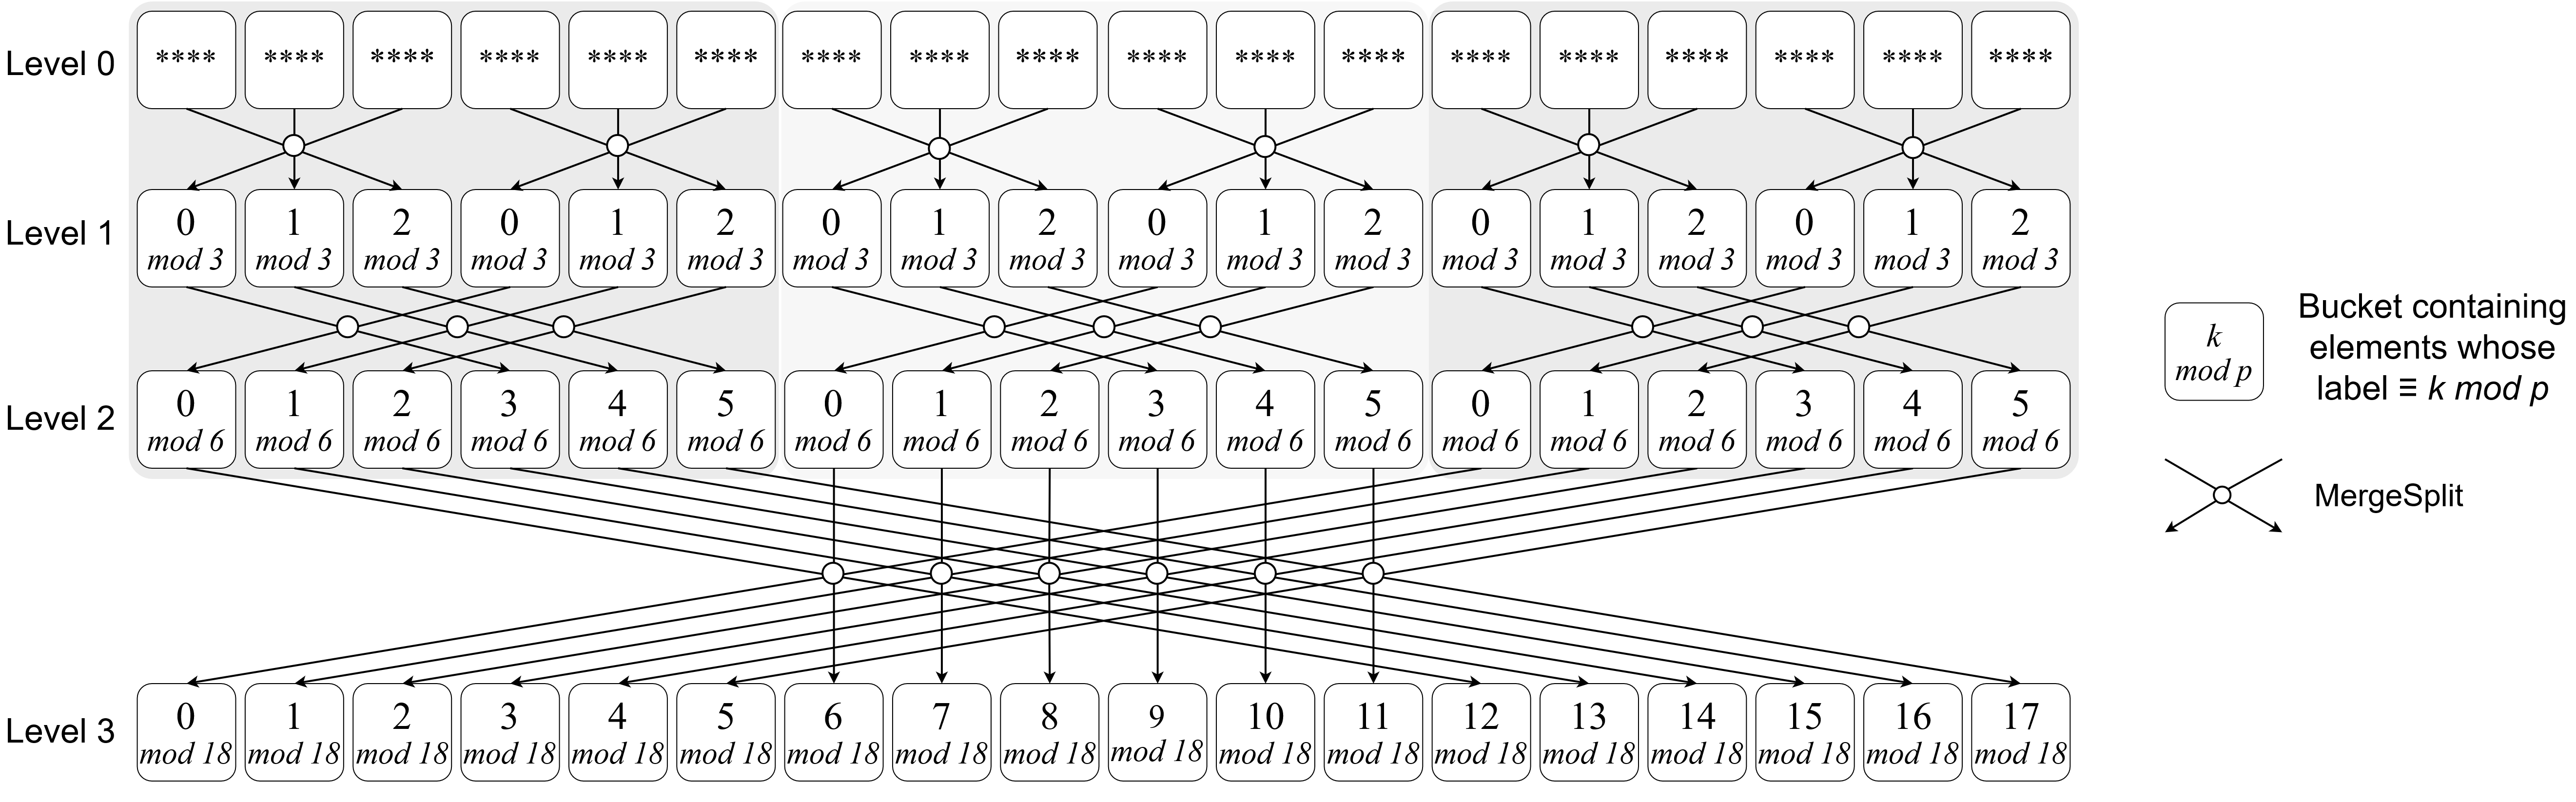
\includegraphics[width=\textwidth]{assets/multi-way-butterfly.png}
    \caption{A 3-level multi-way butterfly network.}
    \label{fig:butterfly}
\end{figure}

As elements are routed to their destination buckets, bitonic sort~\cite{bitonicsort} is executed within each bucket, filter out the filler elements, and remove the tags. At this stage, we have obtained an oblivious random shuffling algorithm. The final step is to run external merge sort~\cite{knuthbook} on all the real elements and get the final sorted array.

When implementing the algorithm in Intel SGX, we need to consider the memory limitations of the SGX enclave, since transferring data across the boundary of the enclave requires expensive cryptographic operations. Naively emulating the butterfly network level by level would incur an extra I/O overhead of $\Theta(\log N)$. Therefore, we want to route elements through multiple levels each time we fetch them into the enclave, as is demonstrated in Figure \ref{fig:batch}. This optimization significantly increases the arithmetic density of the algorithm and thereby improves performance. We can also combine multiple stages of the algorithm in each batch to further reduce the I/O cost. For instance, the first level of the external mergesort can be piggybacked with the last level of the butterfly network. Please refer to \cite{osort} for more details.

\begin{figure}[thbp]
    \centering
    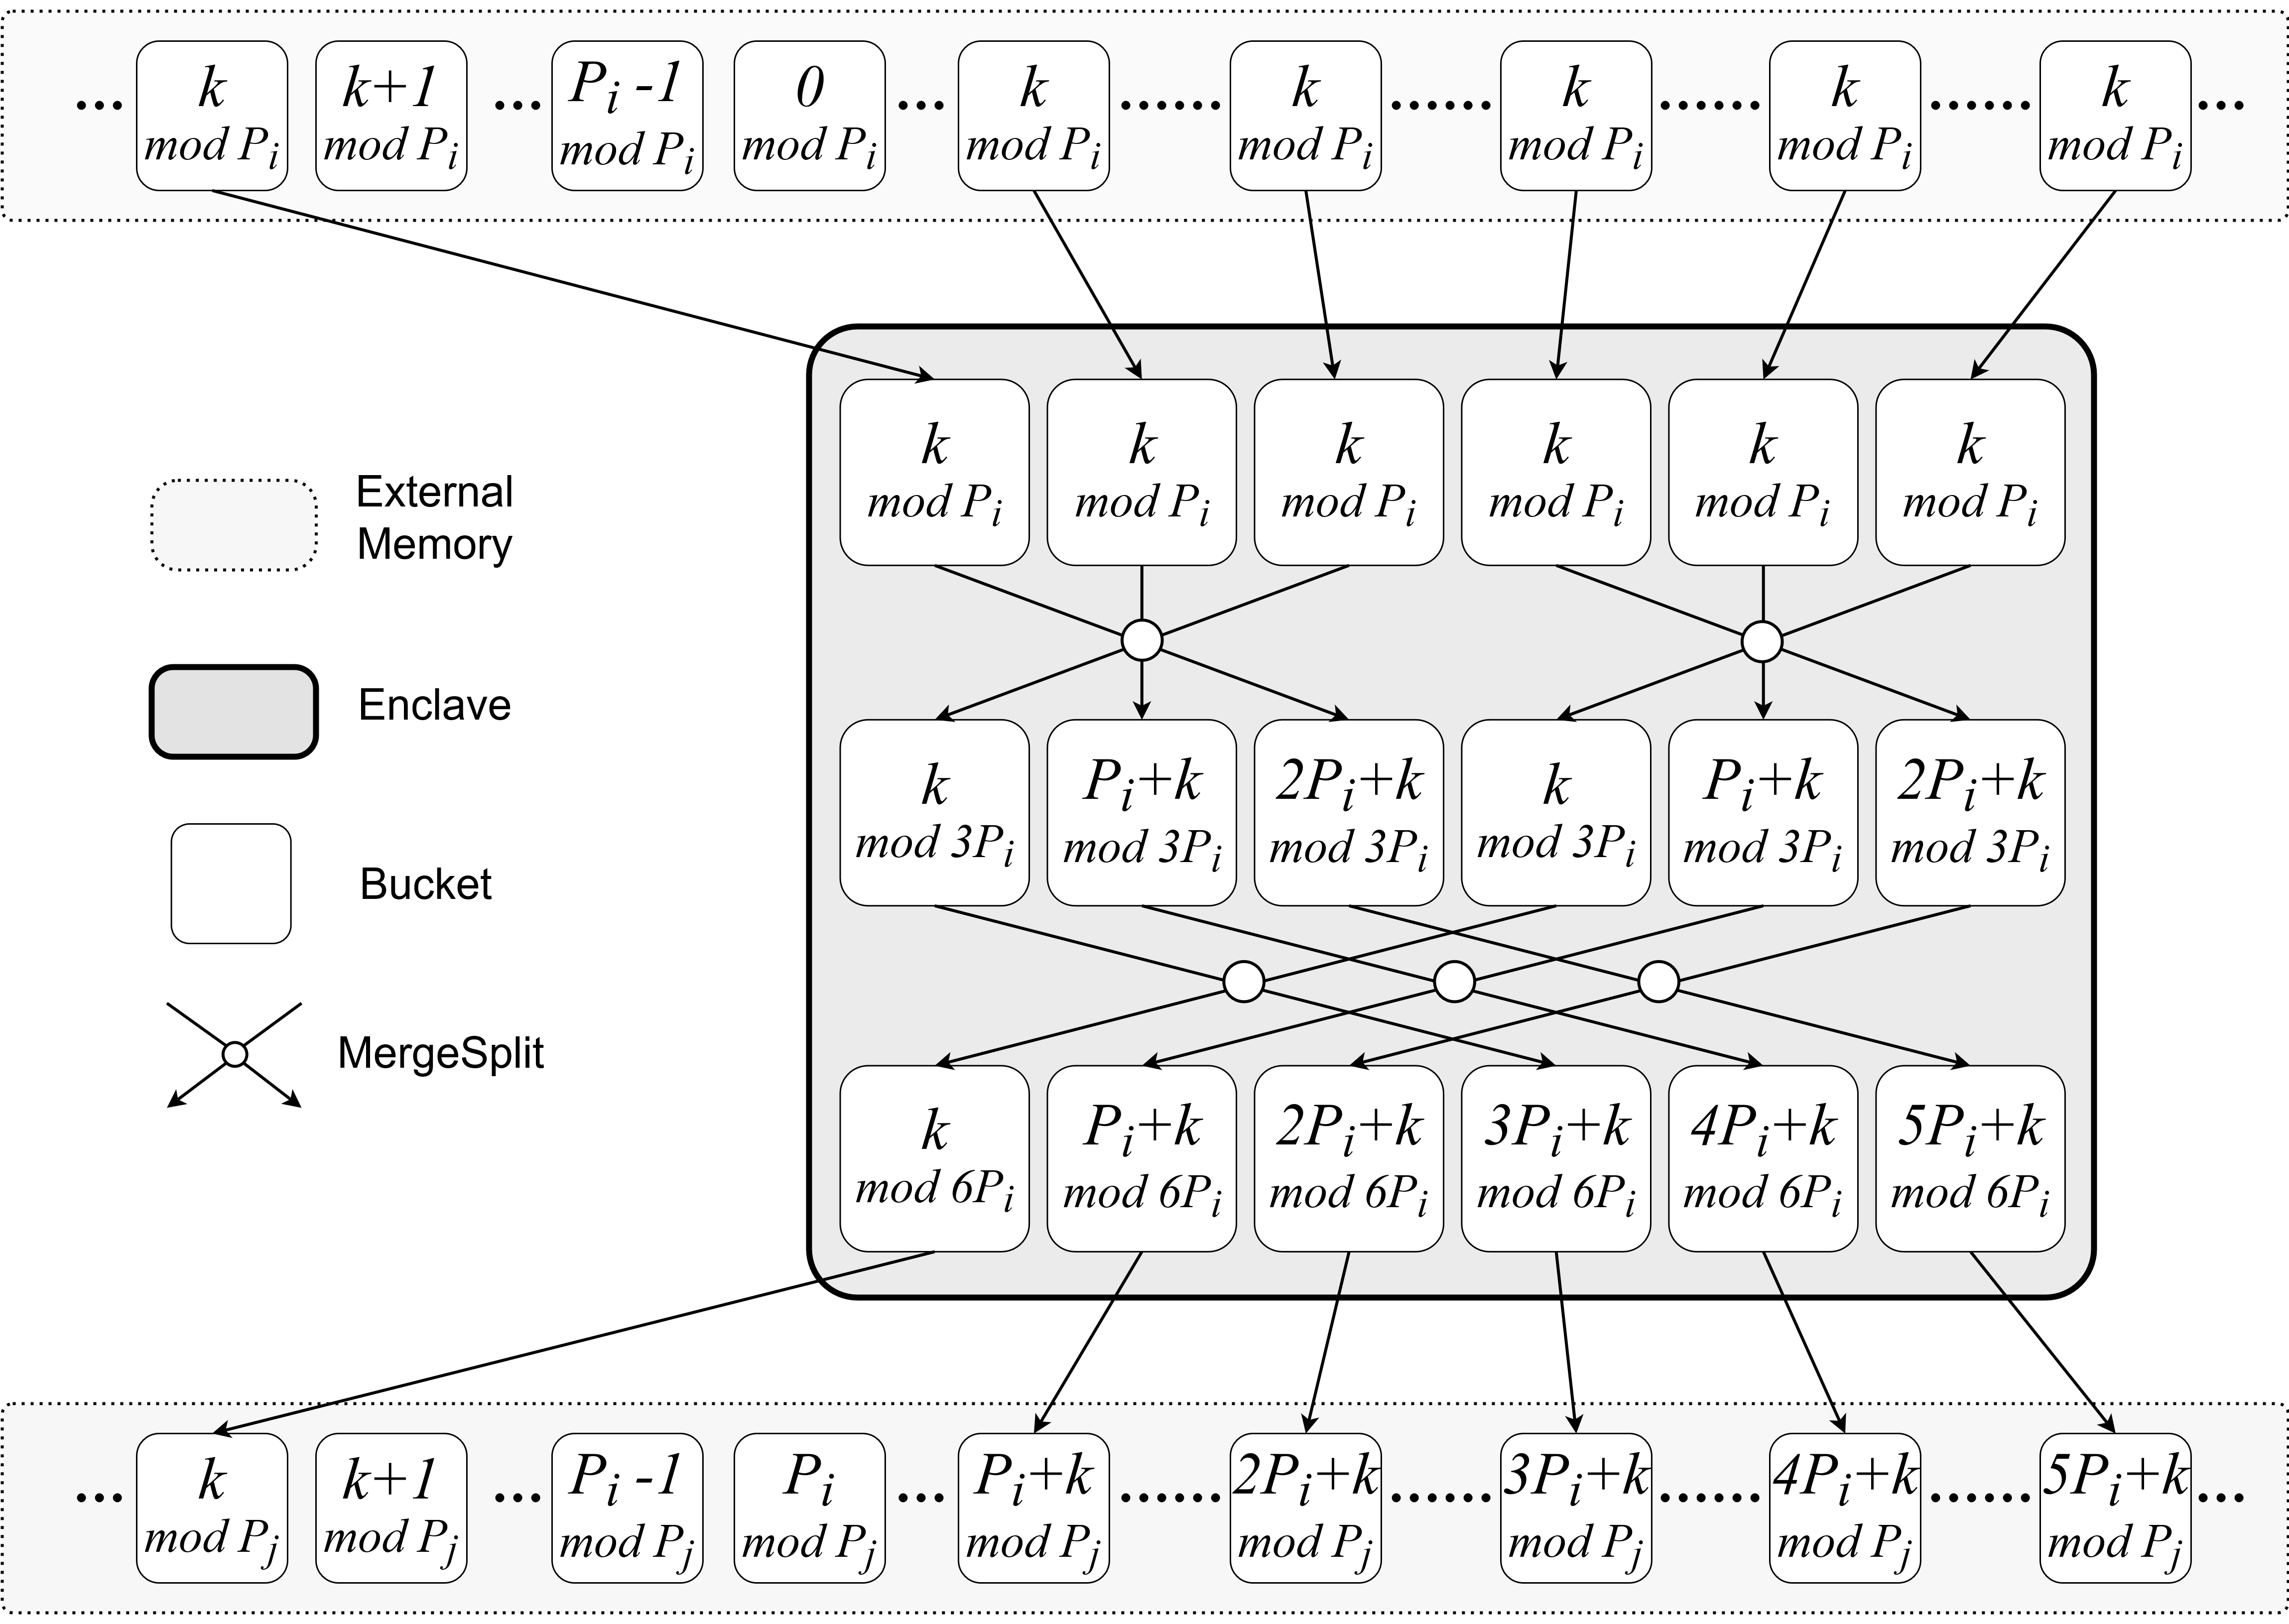
\includegraphics[width=0.8\textwidth]{assets/batch.png}
    \caption{Route elements through multiple levels of butterfly network in each batch.}
    \label{fig:batch}
\end{figure}

\section{Parallelism Abstraction}
\subsection{Parallelism in Butterfly Network}
Emulating the butterfly network is the most time critical part of the algorithm. We observe that merge-split operations on each butterfly network level are independent of each other, and therefore we can parallelize them. In addition, we can also parallelize the bitonic sort within each bucket. Notice that we can only parallelize the merge-split operations within each batch since we cannot access data outside the enclave directly.
\subsection{Parallelism in Multi-way Merge-Split}
The multi-way merge-split operation itself is also parallelizable. It involves a recursive divide-and-conquer algorithm, which can be parallelized by OpenMP. However, we may not achieve a perfect theoretical speedup on the first few recursive calls, since the algorithm involves components that are difficult to parallelize (e.g., searching for an Euler tour on a graph). Moreover, for practical implementation, we need to be careful about the parallelism granularity. Setting the granularity too small would incur too much overhead on thread creation and synchronization.
\subsection{Parallelism in External Merge Sort}
The non-oblivious external merge sort involves two phases. First, we read data into the internal memory (EPC in our case) in batches and sort data in each batch. Second, we merge all the sorted chunks using a priority queue (this step may need to be performed recursively for very large data size and page size).

The first step can be parallelized by running a parallel merge sort in each batch. The priority queue in the second step is more difficult to parallelize. Nevertheless, we can still parallelize the I/O with external memory, as will be elaborated in section \ref{sec:parallelize I/O}.

\subsection{Parallelism in I/O}
\label{sec:parallelize I/O}
We can parallelize the I/O operations with external memory. Specifically, we can parallelize the cryptographic operations when swapping data between the enclave and the untrusted memory. For streaming data, we can apply prefetching and read-back buffers. In theory, when the data exceeds the available physical RAM, we may also swap data to disk in parallel and overlap communication with computation. However, this is more difficult to achieve since disk I/O requires system calls, which are not supported in SGX. Consequently, we must first make {\tt OCALL}s to switch to the untrusted host and perform asynchronous I/O operations.

\subsection{Parallelism in Element Movement}
Our oblivious sorting algorithm assumes that each element consists of a sorting key and a payload. The payload length is not fixed and can be arbitrarily long. We also assumed an indivisible model~\cite{osortsmallkey}, i.e. we cannot separate the payload from the element or perform any computation on the element (such as running compression algorithms). Thus, the payload must be moved along with the sorting key.

Therefore, for elements with large payload, we may parallelize the data movement via SIMD. One particularly interesting case is the oblivious swap operation, i.e., how to conditionally swap two elements without revealing the condition. It turns out that we can apply SIMD to oblivious swap multiple memory words in parallel, as is elaborated in section \ref{sec:simd}.

\subsection{Parallelism in Pseudo-Random Numbers Generation}
The algorithm requires a large number of secure pseudo-random numbers in the shuffling phase. We can parallelize the generation of pseudo-random numbers by using multiple pseudo-random number generators.

\section{Implementation}
\subsection{Overview}
We implemented the algorithm based on the open-source code provided by the authors of the original paper~\cite{osort}, available at \url{https://github.com/odslib/oblsort}. The code is written in C++ and uses the Intel SGX SDK. Below, we describe our modifications to make the program parallel, as well as the major optimizations. While we test the code on a high-end server equipped with 36 cores, 512GB EPC cache and 1TB RAM, our implementation also works for the consumer-grade processors, as well as the virtual machines provided by cloud service providers, which have more limited hardware resources. Figure \ref{fig:parosort} shows a high-level diagram of our implementation on a toy example.

\begin{figure}[htbp]
    \centering
    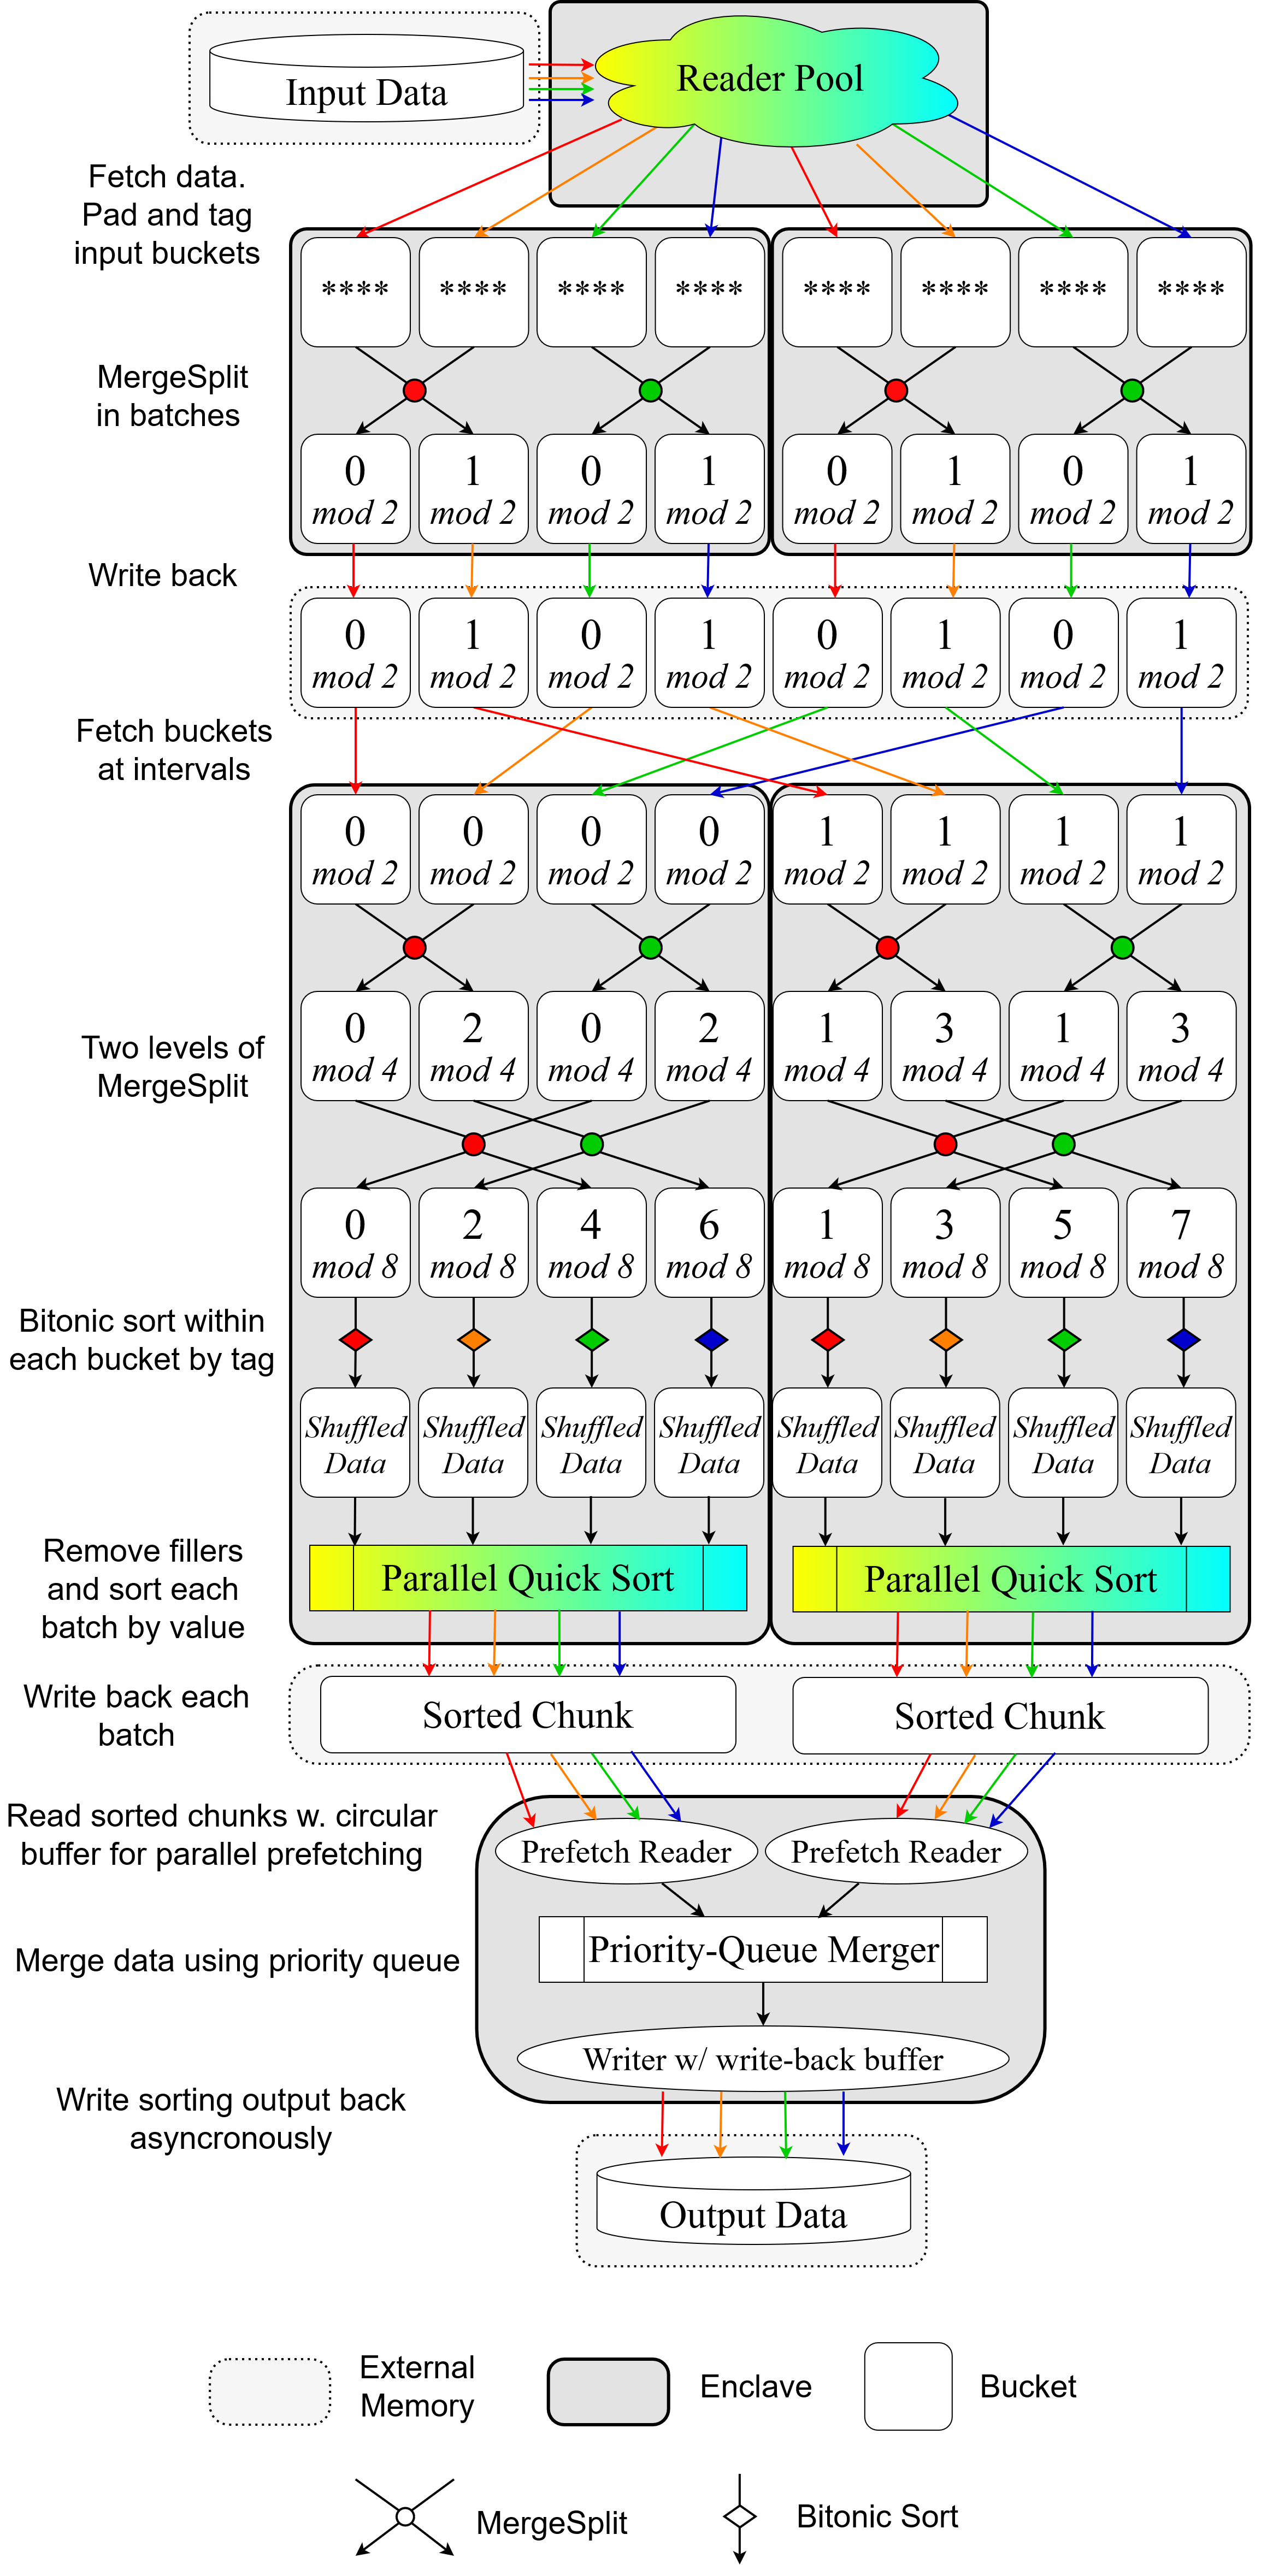
\includegraphics[width=0.72\textwidth]{assets/parosort.png}
    \caption{Diagram of Parallel Oblivious Sort on a toy example. Each color represents a thread. Colorful components are multi-threaded.}
    \label{fig:parosort}
  \end{figure}

\subsection{Parallelize Butterfly Network}
We applied the {\tt \#pragma omp parallel for} directive to parallelize the butterfly network in each batch. Since all the merge-split operations on each level have equal workload, we applied static scheduling to divide the workload evenly among threads and avoid the overhead of dynamic scheduling. We also applied the {\tt \#pragma omp parallel for} directive to parallelize all the bitonic sort operations in each batch.

One modification we made to the original code is to change the butterfly routing schedule from recursive to iterative. In the serial implementation, the butterfly network is divided into two smaller butterfly networks and a merge pass. While the divide and conquer scheduling slightly increases the cache locality of the algorithm, our experiment shows that OpenMP in SGX cannot fully exploit the parallelism in such a recursive program. Therefore, we instead 

To maximize parallelism, we always fetch as many buckets as possible into the enclave in each batch. We also optimized the parameter solver to ensure that there are enough parallel tasks on each butterfly network level (by reducing bucket size and balancing the merge-split ways on each level.)

\subsection{Parallelize External Merge Sort}
\subsection{Parallelize I/O}
We identify three I/O patterns in the algorithm and used different strategies to parallelize them.
\begin{itemize}
    \item {\bf Aligned}
    When each thread reads or writes equal chunks of data that is aligned with the encryption blocks. In this case, the threads have no contention on the encryption blocks, and we can directly apply {\tt \#pragma omp parallel for} to parallelize the I/O operations.

    An example of this case is the swapping of intermediate data in the butterfly network (i.e., all the I/O except reading the initial input and writing the shuffled output). We deliberately set the encryption block size to be equal to the bucket size, and make them perfectly aligned. Therefore, the buckets can be copied into or out of the enclave in parallel.
    \item {\bf Unaligned and Unordered}
    In this case, each thread reads or writes unequal amount of data or the data is not aligned with the encryption blocks, yet we don't care about the order the data being read or written. In this case, we can initiate multiple readers or writers (we let the number match the available threads), each of which is responsible for a roughly equal sized chunk of data that is aligned with the encryption blocks. Moreover, we maintain a central reader/writer pool manager. Each time a thread wants to read or write data, it first requests a reader/writer from the pool manager. The pool manager then assigns a reader/writer to the thread, if available. The reader/writer then reads or writes data in parallel with other readers/writers. When the reader/writer finishes its job, it returns to the pool manager. When a reader/writer is fully consumed, it is destroyed and the thread requests a new reader/writer from the pool manager. The contention is minimized since synchronization with the pool manager only happens when a task begins or ends and when a reader/writer is created or destroyed.

    An example of this case is the input and output of the shuffling phase, since we cannot assume that the input and output page size align with the algorithmic parameters, and the number of data in each task is not perfectly equal (especially for the output since as bucket has a different number of real elements). On the other hand, we don't care about the order of input and output data in a random shuffling algorithm.
    \item {\bf Unaligned and Ordered}
    Finally, we consider the case where each thread reads or writes unequal amount of data or the data is not aligned with the encryption blocks, and we need to read or write data in an ordered and streaming fashion (either one or multiple streams). In this case, we can apply prefetching when reading the data and write-back buffers when writing the data. Since the data is read in a streaming fashion, we can prefetch the data to fill the buffer in parallel. Similarly, we can buffer the data to be written and write them back in parallel when the buffer is full. The buffer size is chosen to be large enough to ensure that the I/O operations are fully parallelized.

    One inefficiency of this approach is that we need an extra copy of the data due to the buffer, and the buffer also consumes some extra EPC space. 

    An example of this case is the input and output of the external merge sort. We applied prefetching when reading the data from multiple sorted chunk, and applied write-back buffers when writing the merged data to external memory.
\end{itemize}
\subsection{Parallelize Element Movement}
\label{sec:simd}
We applied SIMD to parallelize the element movement. Specifically, we used C++ intrinsics to accelerate element-wise oblivious swaps. We incorporated different instruction sets such as AVX512, AVX2, and SSE2 for broader processor compatibility. Specifically, we used the following instructions: 

{\tt \_mm256\_mask\_blend\_pd}, {\tt \_mm256\_set1\_epi32}, {\tt \_mm256\_and\_si256},\\ {\tt \_mm256\_xor\_si256}, {\tt \_mm\_mask\_blend\_pd}, {\tt \_mm\_and\_si128}, {\tt \_mm\_xor\_si128}. 

We observed that the 512-bit wide SIMD operations are actually slower than running two 256-bit operations in series on our processor. This is probably because the 512-bit operations are not fully pipelined due to the limited number of execution ports. Therefore, we used 256-bit operations for the AVX512 instruction set.

Notice that we always pad elements to a multiple of 8 bytes for best performance. Moreover, to minimize the number of SIMD operations, we pad data of size $32k - 8$ bytes to $32k$ bytes, where $k$ is an integer. 

For other places where we need to move elements, we used the {\tt memcpy} function in the C++ standard library, which is already optimized with SIMD for the processor.
\subsection{Parallelize Pseudo-Random Number Generation}
We implemented the pseudo-random number generator with AES counter mode, which features hardware acceleration on our processor. Since the generator is stateful, it is inefficient to use a central pseudo-random generator and synchronize it among multiple threads. Instead, we use multiple pseudo-random generators, each of which is responsible for generating pseudo-random numbers for a subset of the elements.

\subsection{Optimize Memory Utilization}
We want to minimize the memory consumption of the algorithm to maximize the number of elements that can be processed in each batch. Memory fragmentation hence becomes a major concern. While the original serial implementation has addressed this issue, we need to be more careful when parallelizing the algorithm. One specific problem is that each thread requires a temporary buffer to perform the multi-way merge-split operation, and frequently calling new and delete would worsen the memory fragmentation. Another issue is that the OpenMP library also allocates some memory for thread management in the heap, which is not released until the end of the program and causes fragmentation after the algorithm completes. If we run the algorithm a second time, there might not be enough consecutive memory.

To solve these issues, we allocate a large chunk of memory at the beginning of the sorting function and use it as a memory pool. We then implement a custom memory allocator that allocates memory from the pool and releases memory back to the pool. This way, we can avoid memory fragmentation both during and after the execution of the function.
% We have successfully parallelized the oblivious shuffling algorithm in Intel SGX using OpenMP and SIMD.
% Specifically, our key accomplishments include:

% 1. Configured `OpenMP` in the Makefile and set up the multi-threaded environment in the SGX config files.

% 2. Changed the butterfly routing from recursion to iterative, which reduces the overhead of parallel execution. Also, we combined multiple batches into one batch when there's enough memory to increase parallelism.

% 3. Improved the parameter solver to ensure that there are enough parallel tasks on each butterfly network level (by reducing bucket size and balancing the mergesplit ways on each level.)

% 4. Applied `#omp parallel for` to parallelize the butterfly network executions.

% 5. Applied `#omp parallel for` to parallelize I/O operations with external memory.

% 6. Developed a reader/writer pool manager to fetch input and combine the final output, thereby reducing thread contention.

% 7. Separated a central pseudo-random number generator (which uses AES counter mode) to multiple ones to reduce contention.

% 8. Utilized C++ intrinsics to accelerate element-wise oblivious exchange using SIMD. Incorporated different instruction sets such as AVX512, AVX2, and SSE2 for broader processor compatibility.

% 9. Established unit tests on the algorithm outside the enclave for debugging and tuning. Installed Intel vtune software.


\section{Results}
\subsection{Experimental Setup}
We evaluated the performance of our sorting and shuffling algorithms on an Intel Xeon Platinum 8352S processor, which has 36 cores running at 2.2 GHz
frequency. The processor supports Intel SGX v2 and up to 512 GB of EPC cache. Nevertheless, we only uses up to 1.3 GB of EPC cache in our experiments for faster initialization and wider compatibility with consumer-grade processors. The processor supports AVX512, AVX2, and SSE2 instruction sets, and hardware AES acceleration. We used Ubuntu 22.04 as the operating system.

We validate the correctness of our program via unit testing, and evaluated its performance at different thread counts, input size and EPC size.

\subsection{Speedup Results}

\printbibliography
\end{document}